\chapter{Моделирование излучения FBOT}\label{FBOT}

Последние наблюдения открыли новый класс объектов - быстрые голубые оптические транзиенты (FBOT)\cite{Drout2014, Margutti2014, Coppejans2020, Ho2020}. Вместе со слабыми гамма-всплесками они возможно принадлежат к переходному классу объектов между нерелятивистскими сверхновыми и обычными гамма-всплесками. Как показано в работе Шевалье и Ирвина \cite{Chevalier2011} наблюдаемые характеристики вспышки определяются длительностью действия центрального источника энергии выброса и его взаимодействием со внешними слоями взрывающейся звезды. При различных параметрах вспышка будет относиться к разным классам объектов. Известные на данный момент быстрые голубые оптические транзиенты AT2018cow \cite{Margutti2014}, CSS161010 \cite{Coppejans2020}, ZTF2018abvkwla \cite{Ho2020} и AT2020xnd \cite{Ho2021, Bright2021} характеризуются большой светимостью $L > 10^43 эрг/с$, коротким характерным временным масштабом порядка нескольких дней, низкой выброшенной массой эжекты и высокими скоростями.
Рассматриваемы в данной главе объект CSS161010, расположенный в карликовой галактике на расстоянии 150 мегапарсек имеет по оценкам следующие\cite{Coppejans2020} характеристики: скорость эжекты 0.55 c на ранних этапах и около 0.3 c на поздних (порядка одного года), выброшенная масса порядка 0.01-0.1 солнечных масс. ]textcolor{red}{Важнейшей особенностью этих объектов является вид их спектральной плотности излучения, имеющей выраженный максимум и степенные участки, говорящие о наличии синхротронного самопоглощения.}
%почему четвертый был отдельно в статье?


В данной главе будет проведено Particle-in-Cell моделирование ускорения частиц в транс-релятивистской ударной волне со скоростями, характерными для FBOT объектов. По имеющимся распределениям будет расчитано синхротронное излучение и с помощью фитирования наблюдательных данных будут подобраны такие параметры как магнитное поле, концентрация вещества и геометрические характеристики в ударной волне.

\section{Излучение объектов с синхротронным самопоглощением}
Процесс синхротронного излучения хороши известен и описан в классических работах. Но с точки зрения квантовой электродинамки, любому процессу излучения можно так же сопоставить процесс поглощения. Сечение процесса синхротронного самопоглощения описано в работе Гизеллини и Свенсона \cite{Ghisellini1991}. Спектральная плотность мощности излучения единицы объема вещества определеяется формулой
\begin{equation} \label{emission}
I(\nu)=\int_{E_{min}}^{E_{max}} dE \frac {\sqrt {3}{e}^{3}n F(E) B \sin ( \phi)}{{m_e}{c}^{2}}
\frac{\nu}{\nu_c}\int_{\frac {\nu}{\nu_c}}^{\infty }\it K_{5/3}(x)dx,
\end{equation}
где $\phi$ это угол межде вектором магнитного поля и лучом зрения, $\displaystyle\nu_{c}$ критическая частота, определяемая выражением $\displaystyle\nu_{c} = 3 e^{2} B \sin(\phi) E^{2}/4\pi {m_{e}}^{3} c^{5}$, и~$K_{5/3}$ - функция МакДональда.
Коэффициент поглощения для фотонов, распростроняющихся вдоль луча зрения равен
\begin{equation}\label{absorption}
k(\nu)=\int_{E_{min}}^{E_{max}}dE\frac {\sqrt {3}{e}^{3}}{8\pi m_e \nu^2}\frac{n B\sin(\phi)}{E^2}
\frac{d}{dE} E^2 F(E)\frac {\nu}{ \nu_c}\int_{\frac {\nu}{ \nu_c}}^{\infty }K_{5/3}(x) dx.
\end{equation}
Используя эти формулы Шевалье \cite{Chevalier1998} построил модель излучения плоского однородного диска, расположенного перпендикулярно к лучу зрения, с радиусом $R$, толщиной $s$, однородным магнитным полем $B$ и степенной функцией распределения электронов $N(E) = N_0 E^{-p}$. Вместо толщины обычно используется доля излучающего объема $f$, определенная так, что $\pi R^2 s = 4 \pi /3 R^3 f$. При таких предположениях \textcolor{red}{спектральная плотность излучения определяется следующими формулами}
\begin{equation}
I_{\nu}=S(\nu_1)J(\frac{\nu}{\nu_1},p)
{sin(\theta)}^{\frac{p+2}{p+4}},
\end{equation}
где
\begin{equation}
\nu_1 = 2 c_1 {(s c_6 N_0)}^{\frac{2}{p+4}}{B sin(\theta)}^{\frac{p+2}{p+4}}
\end{equation}
\begin{equation}
S(\nu_1)=\frac{c_5}{c_6}{(B sin(\theta))}^{-1/2}{(\frac{\nu_1}{2 c_1})}^{5/2}
\end{equation}
\begin{equation}
J(z,p)=z^{5/2}(1-exp(-z^{(p+4)/2}))
\end{equation}
где $\theta$ - угол между магнитным полем и лучом зрения, $c_1, c_5, c_6$ - константы Пахольчика \cite{Pacholczyk}, зависящие от спектрального индекса электронов.


Измерив спектральную плотность излучения и получив максимум в данный момент времени $F_{max}$, приходящийся на частоту $\nu_{max}$, можно получить размер и магнитное поле в источнике по формулам
\begin{equation}\label{ChevR}
R = {\left( \frac {6 \epsilon_B {c_6}^{p+5}{F_{max}}^{p+6}{
			D}^{2p+12}}{\epsilon_e f \left( p-2 \right) {\pi}^{p+5}{{c_5}}^{p+6}
		{E_1}^{p-2}} \right)} ^{ \frac{1}{p+13} } \frac{2 c_1}{\nu_{max}},
\end{equation}
\begin{equation}\label{ChevB}
B = { \left(\frac {{\epsilon_B}^2 36 {\pi}^{3}{c_5}}{{
			\epsilon_e}^{2}{f}^{2} \left( p-2 \right) ^{2}{{c_6}}^{3}{{E_1}}^{2 p-4}F_{max}{D}^{2}} \right)}
^{\frac{2}{2p+13}}\frac{\nu_{max}}{2 c_1},
\end{equation}
где $D$ - расстояние до источника, $\epsilon_B, \epsilon_e$ - доли энергии в источнике, содержащиеся в магнитном поле и в электронах, $E1$ - энергия, с которой начинается степенное распределение электронов. Таким образом в работах  были оценены параметры источников AT2018cow \cite{Margutti2014}, CSS161010 \cite{Coppejans2020}, ZTF2018abvkwla \cite{Ho2020} и AT2020xnd \cite{Ho2021, Bright2021}. Так же, измеряя радиус источника $R$ в разные моменты времени можно оценить скорость распространения ударной волны.
\section{Particle-in-Cell моделирование }
Для более точного расчета синхротронного излучения оптических транзиентов необходимо знание функции распределения электронов. В перечисленных выше работах используется модель степенного распределения с произвольным параметром - долей энергии в электронах $\epsilon_e$, но как показано в работе \cite{Margalit2021}, тепловые электроны так же могут вносить значительный вклад в излучение. Мы для определения функции распределения электронов в субрелятивистской ударной волне использовали Particle-in-Cell расчеты, выполненные с помощью кода Smilei \cite{Smilei18}, разработанным Деруле и другими. Этот код основан на явной конечно-разностной схеме, с релятивистскими уравнениями движения и с алгоритмом сохранения заряда, предложенным Езиркеповым \cite{Esirkepov}.

Для инициализации ударной волны мы используем распространенный подход - в двумерной симуляции на левой границе по оси $x$ установлена отражающая стенка, с которой сталкивается однородный поток плазмы. На правой границе использованы граничные условия сохраняющие поток. Вдоль перпендикулярного направления $y$ установлены периодические граничные условия. Все вектора, кроме координат частиц - поля и скорости, являются трехмерными, так называемая 2d3v схема. Число ячеек в продольном направлении 
$\displaystyle Nx = 204,800$, в поперечном $\displaystyle Ny = 400$. Размер ячейки $dx = dy = 0.2c/{\omega_e}$ , где $\displaystyle\omega_e$ - плазменная электронная частота $\displaystyle\omega_e = \sqrt{4 \pi n e^2/ m_e}$, $\displaystyle e$ - абсолютная величина заряда электрона, $\displaystyle n$ - концентрация (в коде SMILEI может быть выбрана произвольно, другие величины легко масштабируются), $\displaystyle m_e$ - масса электрона, увеличена для экономии численных ресурсов так, что отношение масс протона и электрона $m_p/m_e = 100$. Начальное магнитное поле $\displaystyle\vec{B}$ лежит в плоскости симуляции под углом $\displaystyle\theta$ к скорости потока. Электрическое поле инициализируется так, чтобы компенсировать силу Лоренца в лабораторной системе $\displaystyle\vec{E} = -\vec{v} \times
\vec{B}/c$. Скорость потока плазмы $\displaystyle v$  is $0.3 c$ 
что соответствует лоренц-фактору $\displaystyle\gamma = 1.05$. Такая скорость соответствует оценкам для выбранного нами транзиента CSS161010 из статьи \cite{Coppejans2020}. Замагниченность потока $\displaystyle\sigma = B^2/4 \pi n \gamma m_p c^2 = 10^{-4}$. С такими параметрами размер области симуляции вдоль оси $\displaystyle x$ соответствует $\displaystyle 500$
гирорадиусам протонов в потоке плазмы $\displaystyle r_g = m_p v c \gamma/e B$, а вдоль оси $\displaystyle y$ одному гирорадиусу. Максимальное время симуляции составляет $\displaystyle 7\times 10^4~\omega_{e}^{-1}$ или около
$\displaystyle 100$ обратных протонных гирочастот. Для концентраций порядка $\displaystyle n\approx
1$~cm$^{-3}$, это время соответствует временам порядка одной секунды, что намного меньше характерного времени активного излучения быстрых оптических транзиентов, а значит такое квазистационарное моделирование применимо к рассматриваемому объекту в каждый отдельный момент времени.

Эффективность ускорения частиц зависит от угла наклона магнитного поля $\displaystyle\theta$,
особенно в случае релятивистских ударных волн \cite{SironiSpitkovsky2009pair, GuoSironi2014_1, Crumley2019, Romansky2018}. Чтобы быть вовлеченной в процесс ускорения Ферми первого рода, частице необходимо удалиться от фронта, и если
она движется вдоль силовых линий магнитного поля, максимальная возможная скорость вдоль оси $\displaystyle x$ равна $\displaystyle c\cos(\theta')$, и для ухода от ударной волны она должна быть больше скорости самой ударной волны $\displaystyle v_{sh}'$ (все величины измерены в системе набегающего потока). Поэтому для квазипоперечных ударных волн, у которых $c \cos(\theta')$ меньше скорости ударной волны $\displaystyle v_{sh}'$ ускорение невозможно. При углах наклона меньших критического, ударная волна способна эффективно ускорять частицы, формировать степенной хвост их функции распределения, как показано на рисунке~\ref{compareelectrons}.
\begin{figure}
	\centering
	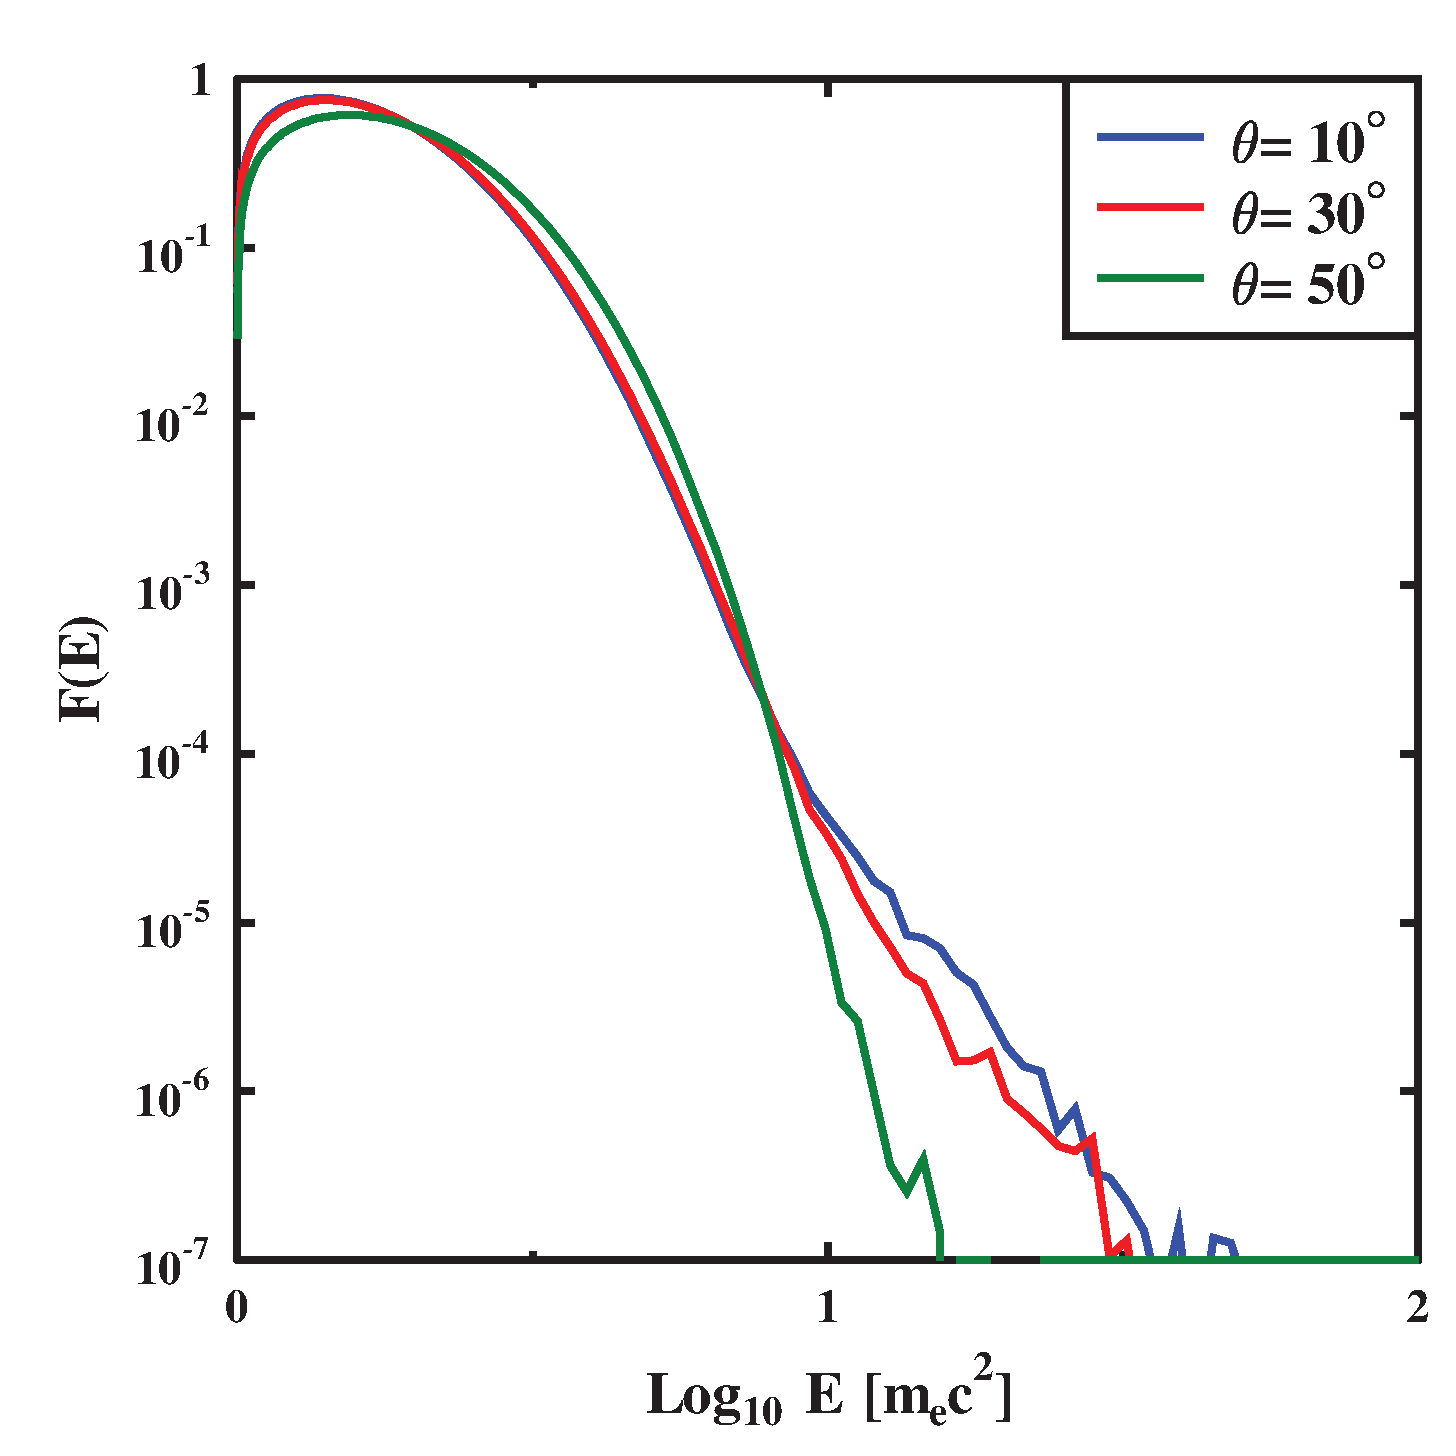
\includegraphics[width=10.5 cm]{compareelectrons2.eps} 
	\caption{Функция распределения электронов за фронтом ударной волны при следующих параметрах: скорость потока \mbox{$v = 0.3~c,$} , магнетизация $\sigma = 0.0002$ при нескольких углах наклона.}
	\label{compareelectrons}
\end{figure}
 
Для дальнейшего моделирования излучения использовалась функция распределения, полученная для угла $\theta = 30^\circ$ градусов (квазипараллельная ударная волна).
 
Из результатов моделирования можно извлечь параметры полученного распределения электронов. За фронтом ударной волны функция распределения электронов имеет сложный вид, но можно выделить две основных компоненты - тепловой пик и степенной хвост на высоких энергиях.
На низких энергиях ($\displaystyle E < 5 m_e c^2$) мы аппроксимируем фунцию распределения с помощью распределения Максвелла-Юттнера, итеративным процессом минимизируя функционал $\displaystyle f(T) = \int_{m_e c^{2}}^{5 m_e c^{2}} (F(E) - F_{mj}(E,T))^{2}dE$, где $\displaystyle F(E)$ функция распределения полученная из моделирования, $\displaystyle F_{mj}(E,T)$ - распределение Максвелла-Юттнера. Таким образом определяется температура, соответствующая тепловому пику. Для высоких энергий ($\displaystyle 20~m_e c^{2} < E < 50~m_e c^{2}$) мы используем линейную регрессию в дважды логарифмических координатах для определения спектрального индекса $p$. Функция распределения электронов за фронтом ударной волны (от 2000 до 5000 ячеек за фронтом) в момент времени $\displaystyle t$ = 70,000~$\omega_{e}^{-1}$ при начальных параметрах $\displaystyle\sigma = 0.0002$, $\theta = 30^\circ$ и ее аппроксимации с \textcolor{red}{температурой $\displaystyle T_e = 5\times 10^{10}$~K} и спектральным индексом $\displaystyle p = 3.6$ изображены на рисунке ~\ref{electrons}.
\begin{figure}
		\centering
		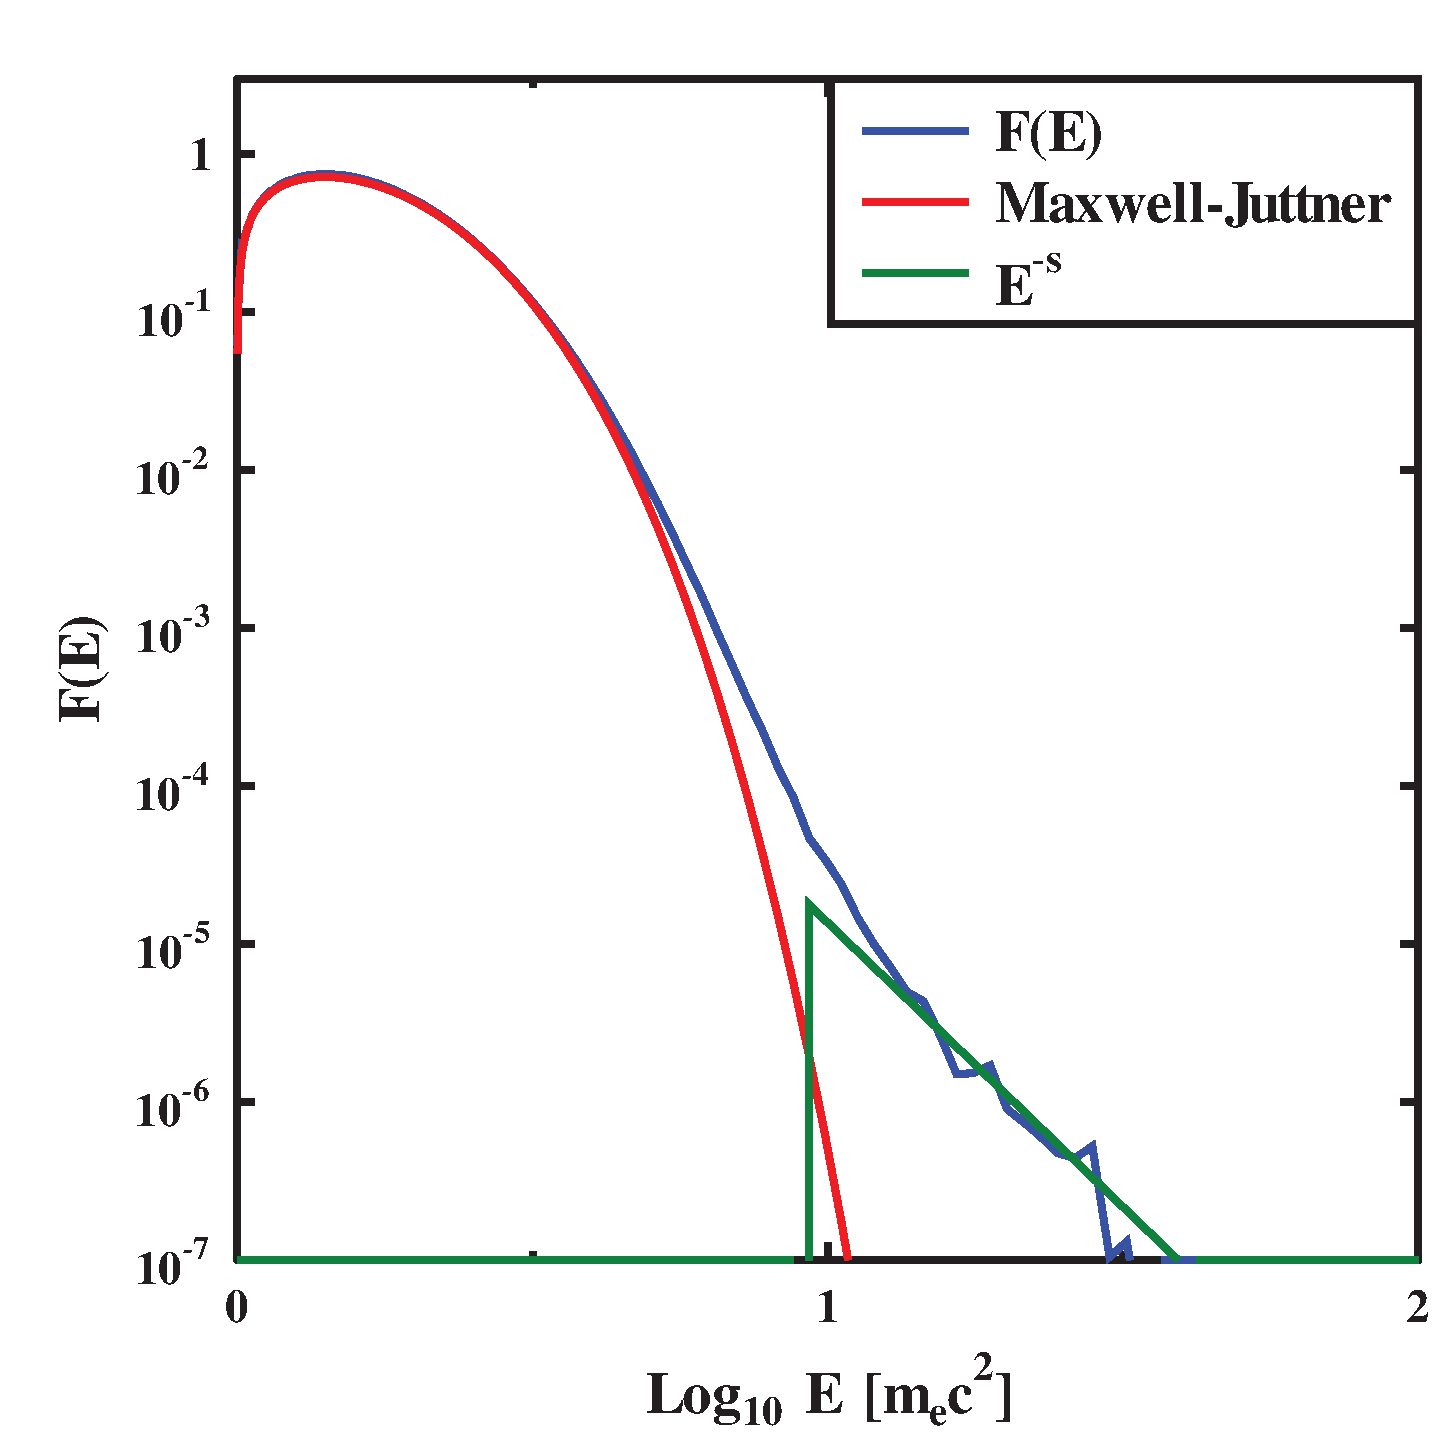
\includegraphics[width=10.5 cm]{electrons.eps} 
		\caption{Функция распределения электронов за фронтом ударной волны при начальных параметрах $v = 0.3~c,$ $\sigma = 2\times10^{-4}$ и $\theta = 30^{\circ}$.}
		\label{electrons}
	\end{figure}

\section{Расчёт излучения}




\section{Результаты}




\FloatBarrier
\section{Заключение}
 

Получены следующие результаты:
\begin{enumerate}
\item 
\item 
\end{enumerate}


\clearpage